\begin{frame}
  \frametitle{Cascaded Differential Equations}
  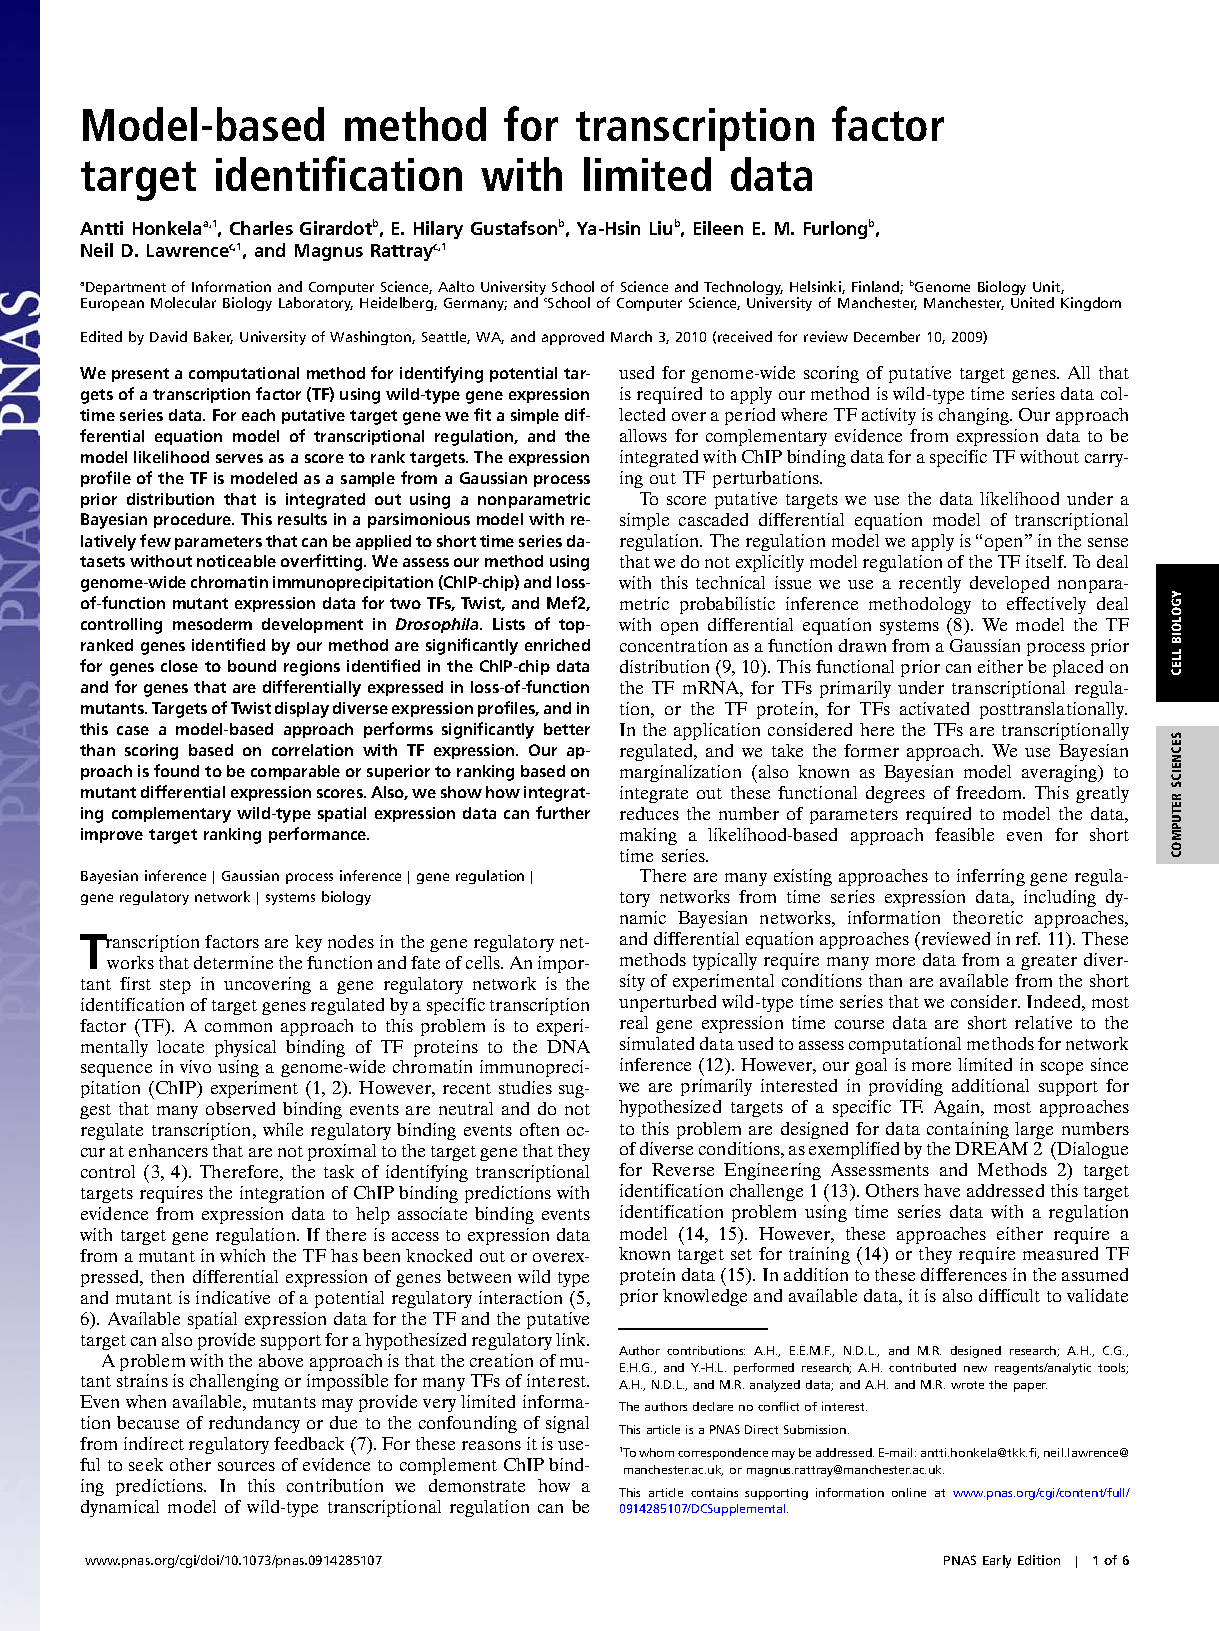
\includegraphics[trim=0cm 20cm 3cm 1cm, clip=true, width=\textwidth]{../../../gpsim/tex/disim_pnas/pnas_paper}
\end{frame}

\begin{frame}
  \frametitle{Cascaded Differential Equations}

  \begin{flushright}
    \textbf{\citep{Honkela:modelbased10}}
  \end{flushright}
  \begin{itemize}
  \item Transcription factor protein also has governing mRNA.
  \item This mRNA can be measured.
  \item In signalling systems this measurement can be misleading because it
    is activated (phosphorylated) transcription factor that counts.
  \item In development phosphorylation plays less of a role.
  \end{itemize}

\end{frame}

\subsection{Drosophila Mesoderm Development}
\begin{frame}
  \frametitle{Drosophila \emph{Mesoderm} Development}

  \textbf{Collaboration with Furlong Lab in EMBL Heidelberg.}
  \begin{itemize}
  \item Mesoderm development in Drosophila melanogaster (fruit fly).
  \item Mesoderm forms in triplobastic animals (along with ectoderm and endoderm). Mesoderm develops into muscles, and circulatory system.
  \item The transcription factor Twist initiates Drosophila mesoderm development, resulting in the formation of heart, somatic muscle, and other cell types.
  \item Wildtype microarray experiments publicly available.
  \item Can we use the cascade model to predict viable targets of Twist?
  \end{itemize}

\end{frame}


\begin{frame}
  \frametitle{Cascaded Differential Equations }

  \begin{flushright}
    \textbf{\citep{Honkela:modelbased10}}
  \end{flushright}

  We take the production rate of active transcription factor to be given
  by 
  \begin{align*}
    \frac{\dif \tfConcentration\left(t\right)}{\dif t} & =\sigma \tfMrnaConcentration\left(t\right)-\delta \tfConcentration\left(t\right)\\
    \frac{\dif \mrnaConcentration_{j}\left(t\right)}{\dif t} & =\basalRate_{j}+\sensitivity_{j}\tfConcentration\left(t\right)-\decayRate_{j}\mrnaConcentration_{j}\left(t\right)
  \end{align*}
  The solution for $\tfConcentration(t)$, setting transient terms to zero, is 
  \[
  \tfConcentration(t)=\sigma\exp\left(-\delta t\right)\int_{0}^{t}\tfMrnaConcentration(u)\exp\left(\delta u\right)\text{d}u\ .
  \]



\end{frame}

\input{../../../kern/tex/talks/disimcovariance.tex}

\setbeamercovered{invisible}
\begin{frame}
  \frametitle{Joint Sampling of $\tfMrnaConcentration\left(t\right)$, $\tfConcentration\left(t\right)$, and $\mrnaConcentration\left(t\right)$ }
  \begin{itemize}
  \item {\texttt{disimSample}}%
    \begin{figure}
      \multiinclude[graphics={width=0.5\textwidth},start=1,end=4,format=pdf]{../../../kern/tex/diagrams/disimSample}
%       \includegraphics<1>[width=0.5\textwidth]{../../../kern/tex/diagrams/disimSample1}
%       \includegraphics<2>[width=0.5\textwidth]{../../../kern/tex/diagrams/disimSample2}
%       \includegraphics<3>[width=0.5\textwidth]{../../../kern/tex/diagrams/disimSample3}
%       \includegraphics<4>[width=0.5\textwidth]{../../../kern/tex/diagrams/disimSample4}
%      \includegraphics<5>[width=0.5\textwidth]{../../../kern/tex/diagrams/disimSample5}
%      \includegraphics<6>[width=0.5\textwidth]{../../../kern/tex/diagrams/disimSample6}
%      \includegraphics<7>[width=0.5\textwidth]{../../../kern/tex/diagrams/disimSample7}
%      \includegraphics<8>[width=0.5\textwidth]{../../../kern/tex/diagrams/disimSample8}

      \onslide<1->\caption{ {\small Joint samples from the ODE covariance,
          \textcolor{blue}{\emph{blue}: $\tfMrnaConcentration\left(t\right)$ (mRNA of TF)},
          \textcolor{black}{\emph{black}: $\tfConcentration\left(t\right)$ (TF concentration)},
          \textcolor{red}{\emph{red}: $\mrnaConcentration_{1}\left(t\right)$ (high
            decay target)} and \textcolor{green}{\emph{green}:
            $\mrnaConcentration_{2}\left(t\right)$ (low decay target)}}}.
      
    \end{figure}
    
  \end{itemize}
  
\end{frame}
\setbeamercovered{transparent}

\subsection{Results for Twist Transcription Factor}

\begin{frame}
\frametitle{Twist Results}
\begin{itemize}
\item Use mRNA of Twist as driving input.
\item For each gene build a cascade model that forces Twist to be the only TF.
\item Compare fit of this model to a baseline (\emph{e.g.} similar model but sensitivity zero).
\item Rank according to the likelihood above the baseline. 
\item Compare with correlation, knockouts and time series network identification (TSNI) \citep{DellaGatta:direct08}.
\end{itemize} 
\end{frame}
\begin{frame}
  \frametitle{Results for Twi using the Cascade model}
  % \begin{columns}[c]%{}
  
  
  %   \column{2 in}
  
  %     %   
  \begin{figure}
    \begin{center}
      \includegraphics<1>[width=8cm]{../../../gpsim/tex/diagrams/gpdisim_model_twi_FBgn0002526} 
      \includegraphics<2>[width=8cm]{../../../gpsim/tex/diagrams/gpdisim_model_twi_FBgn0003486}
      \includegraphics<3>[width=8cm]{../../../gpsim/tex/diagrams/gpdisim_model_twi_FBgn0011206}
      \includegraphics<4>[width=8cm]{../../../gpsim/tex/diagrams/gpdisim_model_twi_FBgn0030955}
      \includegraphics<5>[width=8cm]{../../../gpsim/tex/diagrams/gpdisim_model_twi_FBgn0031907}
      \includegraphics<6>[width=8cm]{../../../gpsim/tex/diagrams/gpdisim_model_twi_FBgn0035257}
      \includegraphics<7>[width=8cm]{../../../gpsim/tex/diagrams/gpdisim_model_twi_FBgn0039286}
    \end{center}
    \caption{Model for flybase gene identity FBgn00\only<1>{02526}\only<2>{03486}\only<3>{11206}\only<4>{309055}\only<5>{31907}\only<6>{35257}\only<7>{39286}.}
  \end{figure}
  
  
  % 
  % \end{columns}%{}
  
\end{frame}


\frame{
  \frametitle{Evaluation methods}

  \begin{itemize}
  \item Evaluate the ranking methods by taking a number of top-ranked
    targets and record the number of
    ``positives''~\citep{Zinzen2009}:
    \begin{itemize}
    \item targets with ChIP-chip binding sites within 2 kb of gene
    \item (targets differentially expressed in TF knock-outs)
    \end{itemize}
  \item Compare against
    \begin{itemize}
    \item Ranking by correlation of expression profiles
    \item Ranking by $q$-value of differential expression
      in knock-outs
    \end{itemize}
  \item Optionally focus on genes with annotated expression in
    tissues of interest
  \end{itemize}
}

\frame{
  \frametitle{Results}

  \begin{center}
    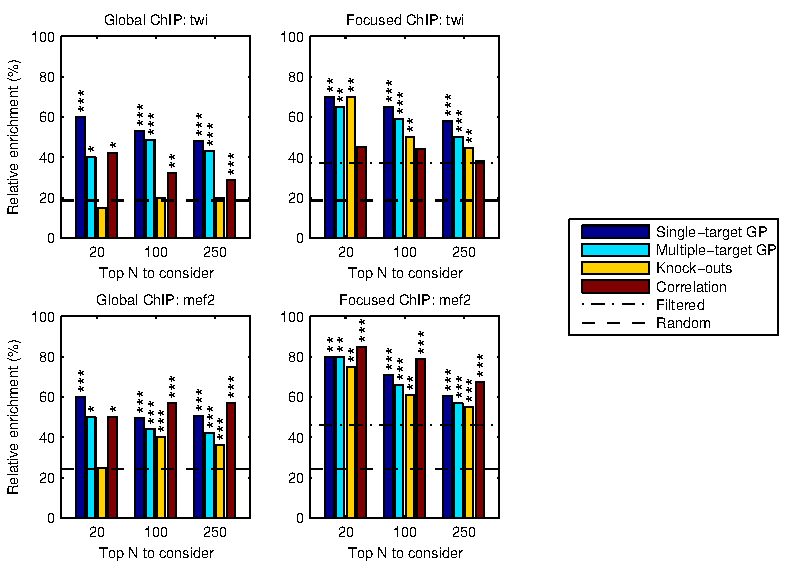
\includegraphics[width=\textwidth,trim=0mm 3mm 0mm 0mm]{../../../gpsim/tex/diagrams/dros_comparison_for_slides_2010-05-07} \\
    {\tiny '***': $p < 0.001$, '**': $p < 0.01$, '*': $p < 0.05$}
  \end{center}
}

% \begin{frame}
%   \frametitle{Results of Ranking}
%   \begin{figure}
%     \includegraphics<1>[width=8cm]{../../../gpsim/tex/diagrams/neil_insitu_validation_2009-06-23}
%     \includegraphics<2>[width=8cm]{../../../gpsim/tex/diagrams/neil_chip_validation_2009-06-23}
%     \caption{Percentage enrichment for top $N$ targets for \only<1>{relevant terms in \emph{Drosophila} in situs}\only<2>{ChIP-chip confirmed targets}.}
%   \end{figure}
% \end{frame}
\begin{frame}
  \frametitle{Summary}
  \begin{itemize}
  \item Cascade models allow genomewide analysis of potential targets given only expression data.
  \item Once a set of potential candidate targets have been identified, they can be modelled in a more complex manner. 
  \item We don't have ground truth, but evidence indicates that the approach \emph{can} perform as well as knockouts.
  \end{itemize}
\end{frame}
